\chapter{Architektur}

\section{Der Hub}
\sectionauthor{\leonard}

Der \emph{Spielehub} ist der zentrale Zugangspunkt, und auch das Erste, was der
Nutzer sieht. Er ist in 3 Teile aufgespalten und besitzt eine seitliche
Navigationsleiste(\emph{Navigation-Drawer}). Jedes Teil ist dabei ein
\textbf{Fragment}. Der Hub besteht aus dem \emph{Spielehub}, welcher die
Spielstände als Liste hält, und den \emph{Kartenspielen} und \emph{Brettspielen}.

\begin{infobox}[frametitle=Fragment]
Dies kann man wie eine Sub-\textbf{Activity} sehen, welche in einer
\textbf{Activity} platziert wird. Sie ist an den \textbf{Lifecycle} der
\textbf{Activity} gekoppelt, aber hat auch einen eigenen. Es können
mehrere Fragmente innerhalb einer \textbf{Activity} existieren. Fragmente werden
in ein \textbf{FrameLayout} gesetzt.
\end{infobox}

\begin{figure}[h]
	\centering
	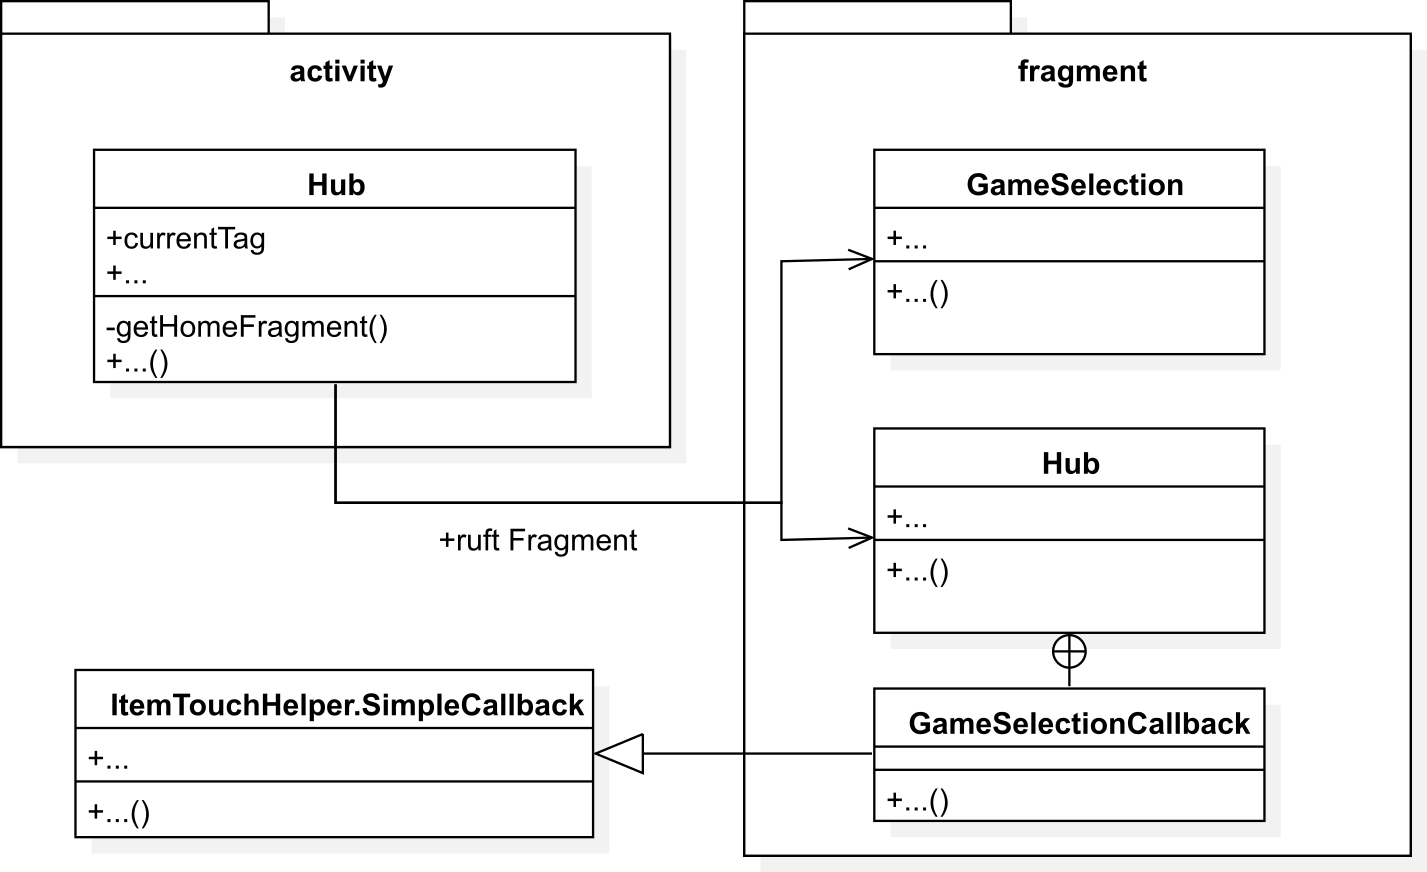
\includegraphics[width=1.0\textwidth]{resources/hub/Hub}
	\caption{Der Hub}
\end{figure}

\section{Die Spielstände}
\sectionauthor{\leonard}

Da man Spiele nicht immer in einem Zug durchspielt und man zwischendurch Pause
macht, ist es sinnvoll, das Speichern und Laden der Spiele zu ermöglichen. Für
diese Funktion sind die Klassen \code{SavegameStorage}, \code{Savegame} und
\code{SavegameAdapter} zuständig.

\subsection{Klassen}

\code{Savegame} ist das Spielstand-Objekt, welches alle Daten speichert, die
nötig sind, um ein Spiel fortsetzen zu können. Jedes \code{Savegame} ist dabei
einzigartig.

\code{SavegameStorage} kümmert sich um das Speichern und Laden der
\code{Savegame} Objekte. Diese werden als Liste serialisiert und auf dem Gerät
gespeichert.

\code{SavegameAdapter} erstellt aus den gepeicherten \code{Savegame} Objekten;
für jeden Spielstand eine Karte, welche im Startbildschirm in einer Liste
angezeigt wird. Die Klasse ist etwas komplizierter aufgebaut als die anderen.

\begin{figure}[h]
	\centering
	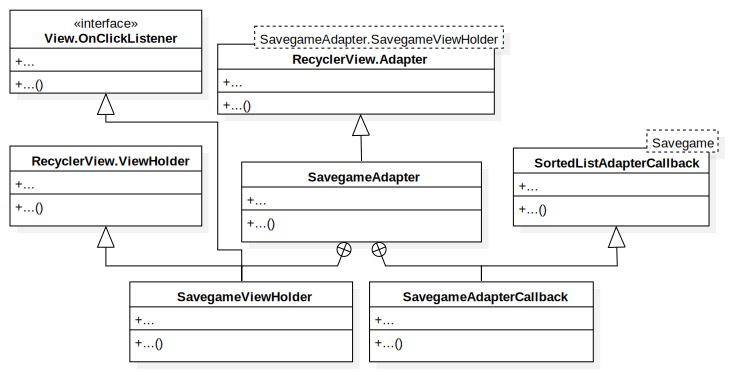
\includegraphics[width=1.0\textwidth]{resources/savegamestorage/SavegameAdapter}
	\caption{Spielstand SavegameAdapter}
\end{figure}

\code{SavegameViewHolder} \& \code{SavegameAdapterCallback} sind zwei innere
Klassen. Erstere erbt von \code{RecyclerView.ViewHolder} und implementiert
gleichzeitig das Interface \code{View.OnClickListener}. Zweitere erbt von
\code{SortedListAdapterCallback<Savegame>}. \code{SavegameAdapter} erbt von
\code{RecyclerViewAdapter<SavegameAdapter.SavegameViewHolder>}

\subsection{Aufbau}
\subsectionauthor{\frank}

Wenn ein Spiel gespeichert oder geladen werden soll, geschieht dies durch einen
Aufruf der Instanz \code{SavegameStorage}. Um hier nicht mehrmals neuen Code,
welche alle Spiele gemeinsam haben, schreiben zu müssen, haben wir diese
Aufgabe an die Klasse \code{GameActivity} abgegeben. Da nun jedes Spiel von
\code{GameActivity} erben soll, müssen dadurch unter anderem zwei abstrakte
Methoden -- zum Speichern und Laden -- implementiert werden.
\code{onSaveGame(Bundle)} respektive \code{onLoadGame(Bundle)}. Diese Methoden
arbeiten jeweils mit einem \textbf{Bundle}, welchem die für einen
Speicherzustand nötigen Informationen übergeben beziehungsweise entnommen
werden können.

\begin{infobox}[frametitle=Bundle]
Dies ist ein Objekt welches verschiedene Datentypen, wie zum Beispiel:
\emph{String, int} oder \emph{long}, mit \emph{String-Keys mapped} und hochperfomant
für \emph{Interprozesskommunikation} ist.
\end{infobox}

Das der Methode \code{onSaveGame} übergebene Bundle kann mit Methoden wie
\code{.putString} oder \code{.putStringArrayList} mit gefüttert werden.
Anschließend werden die gespeicherten Werte weiterverarbeitet und
abgespeichert. Das bedeutet, falls das Bundle unangetastet bleibt, kann
signalisiert werden, dass kein Speichern gewünscht ist, und so der Spielstand
nicht überschrieben wird. Dies ist sehr hilfreich, wenn ein Spiel gestartet,
der Zustand diesen aber nicht verändert wurde. So wird verhindert, dass die
Spielstandliste mit Startaufstellungen von Spielen überfüllt wird. Support für
das Löschen eines Spielstandes ist an dieser Stelle zum aktuellen Zeitpunkt
noch nicht vorhanden.

\let\thefootnote\relax\footnote{Ein Klassendiagramm der Spielstände, ist im Anhang zu finden.}

\section{Einstellungen und Info}
\sectionauthor{\leonard}

Da der Nutzer gerne seine App selbst ein wenig gestalten will, ist es ratsam
Einstellung zu haben. Ob farbliche Akzente oder die Schwierigkeit des
Gegenspielers, der Nutzer ist glücklicher wenn er bestimmen darf. Deswegen
haben wir Einstellungen implementiert und außerdem noch eine Informationsseite,
welche für den Nutzer von Interesse sein könnte. 

\begin{figure}[h]
	\centering
	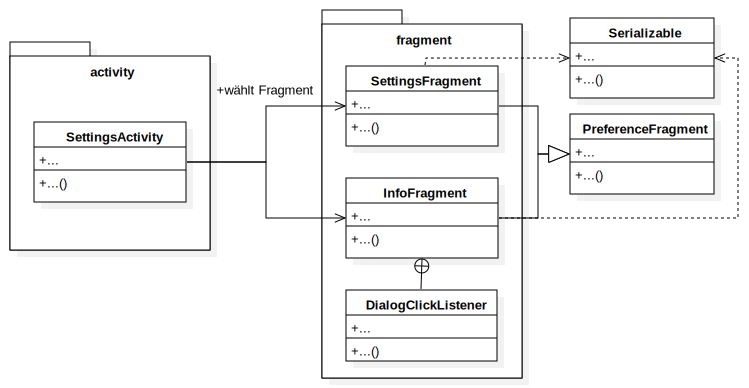
\includegraphics[width=1.0\textwidth]{resources/settingsandinfo/SettingsAndInfo}
	\caption{Einstellungen und Info}
\end{figure}

Die \code{SettingsActivity} wählt das jeweilige \textbf{Fragment}, welches
angezeigt werden soll. \code{SettingsFragment} ist für die Einstellungen und
\code{InfoFragment} für die Informationsseite zuständig. Beide erben von
\code{PreferenceFragment}und implementieren das Interface
\code{Serializable}. Da \emph{Info} einige Dialoge anzeigen muss, enthält es
die innere Klasse \code{DialogClickListener}.

